\documentclass[journal]{IEEEtran}

\usepackage{amsmath,amssymb}
\usepackage{graphicx}
\usepackage{booktabs}
\usepackage{multirow}
\usepackage{tikz}
\usetikzlibrary{arrows.meta,positioning,shapes.geometric}
\usepackage{algorithm}
\usepackage{algpseudocode}
\usepackage{url}
\usepackage{xcolor}

\newcommand{\todo}[1]{\textcolor{red}{[TODO: #1]}}

\begin{document}

\title{Certified Numeric Verification: Guaranteed-Error Fact-Checking of\\ Numeric Claims over Tables with Automated Human Escalation}

\author{Mohd.~Aatir, Prafful Gupta, Prashant Kumar Singh, \todo{Member 4}\\
\textit{Department of Computer Applications (MCA), KIET Group of Institutions}}

\maketitle

\begin{abstract}
Large language models verify numeric claims about tables unreliably: they
miscount rows, mis-sum columns, and get comparisons wrong, yet the sentences
they produce for a wrong numeric claim are nearly indistinguishable, in
meaning, from the sentence for the correct one. Citation-based fact-checking
does not help here, because aggregated numbers -- counts, totals, averages --
are not written anywhere in the source table to cite. We present Certified
Numeric Verification (CNV), a system that (1) introduces
NumNear-TabFact, a large, programmatically constructed and label-flip-verified
benchmark of minimally perturbed numeric near-miss claims built from
TabFact, showing that such near-misses have a mean cosine similarity of
$0.961$ (91.2\% of pairs above $0.9$) to their true counterparts under a
standard sentence embedding model while being factually opposite; (2)
replaces free-text LLM verdicts with \emph{execution-agreement confidence}:
an LLM translates a claim into an executable check over the table, sampled
$K$ times, and confidence is the agreement among the $K$ executed verdicts;
and (3) applies split-conformal risk control to that confidence so that,
among the claims the system answers, the error rate is guaranteed, with high
probability, not to exceed a chosen $\alpha$ -- every claim below threshold
is instead routed to a human reviewer through an automated RPA workflow. We
evaluate on the full numeric subset of TabFact's test split (11{,}400
claims) and on NumNear-TabFact (5{,}474 test-derived near-miss claims);
\todo{full-run accuracy/coverage/risk numbers pending -- large-scale
evaluation in progress, see Section~\ref{sec:results}}. Our
contribution targets SDG 16 (public access to reliable information) and, as
an institutional deployment, SDG 4 (educational information).
\end{abstract}

\begin{IEEEkeywords}
table fact verification, numerical reasoning, conformal prediction, selective
prediction, program-aided reasoning, robotic process automation, large
language models
\end{IEEEkeywords}

\section{Introduction}
\label{sec:intro}

Large language models (LLMs) are increasingly used to answer factual
questions about tabular data -- fee structures, exam results, budgets,
schedules -- yet they remain unreliable at exactly the kind of reasoning
tables demand: counting rows, summing a column, computing an average,
comparing two cells. A claim like ``the total fee for MCA semester~1 is
95{,}000'' and the claim ``the total fee for MCA semester~1 is 99{,}000''
differ by a single number, but one is true and one is false. An LLM asked to
verify either claim in free text can silently get the arithmetic wrong and
report high confidence in the wrong answer, with no trace of how it arrived
there.

Citation-based fact-checking, the standard defense against LLM
hallucination, does not solve this problem. A citation points to a passage
that supports a claim; but the number ``95{,}000'' in the example above is
not written anywhere in the source table -- it is the \emph{sum} of a
tuition-fee cell and a hostel-fee cell. There is no sentence to cite for a
count, a total, or an average; the fact must be \emph{computed}, and citing
the table itself does nothing to tell a reader whether the computation was
done correctly. Worse, because a wrong numeric claim is semantically almost
identical to the correct one -- same subject, same units, same sentence
structure, one digit different -- similarity-based and retrieval-based
verifiers, which work by checking whether a claim is entailed by *similar*
evidence, cannot distinguish the two: both claims are equally ``similar'' to
the table.

This near-miss problem is not hypothetical. In
Section~\ref{sec:nearmiss} we construct NumNear-TabFact, a large set of
claims built by changing exactly one number in a true TabFact claim just
enough to flip its label, and show that the average cosine similarity
between a true claim and its near-miss, under a standard sentence embedding
model, is $0.961$, with $91.2\%$ of pairs above $0.9$
similarity. \todo{LLM-only accuracy on these near-misses vs.\ originals is
being measured at full scale (Section~\ref{sec:results}); pilot-scale
evidence is discussed there.} A system that cannot distinguish these pairs
by meaning alone has no choice but to compute the disputed number directly.

Our approach is to stop asking the LLM to be the arithmetic engine and
instead ask it to be a \emph{translator}: given a claim and a table, the LLM
emits a small, executable ``check'' -- a JSON program with a row filter, a
target column, and an operation such as \texttt{count}, \texttt{sum},
\texttt{avg}, or \texttt{compare} -- and a Python/pandas executor computes
the verdict deterministically. Because LLM outputs are still stochastic, we
sample $K$ such checks per claim and use the \emph{agreement} among their
executed verdicts as a confidence signal: a claim where all $K$ independently
generated, independently executed checks agree is one we can trust more than
a claim where they split. We then calibrate this confidence with
split-conformal risk control (Section~\ref{sec:method}), which lets us fix a
target error rate $\alpha$ in advance -- $\alpha\in\{0.02, 0.05, 0.10\}$ in
our experiments -- and derive an agreement threshold such that, among claims
the system chooses to answer, the empirical error rate is guaranteed, with
high probability under exchangeability, not to exceed $\alpha$. Every claim
below threshold abstains and is routed automatically to a human reviewer
through a UiPath robotic process automation (RPA) workflow, with a
quantified, bounded review workload rather than an ad hoc escalation rule.

\textbf{Contributions.}
\begin{itemize}
\item \textbf{C1 -- NumNear-TabFact.} A large numeric near-miss benchmark
built programmatically (no LLM calls) from TabFact's train and test splits,
by matching a number in a true claim to a uniquely occurring value in its
table (a raw cell or a computed aggregate) and perturbing it -- off-by-one,
digit swap, magnitude change, or round-number change -- while verifying,
against the table, that the label actually flips.
\item \textbf{C2 -- Execution-agreement confidence.} A JSON check language
executed deterministically over the table, sampled $K$ times per claim, with
confidence defined as agreement among the $K$ executed verdicts; invalid or
failing checks count as abstain votes.
\item \textbf{C3 -- Conformal risk control.} Split-conformal calibration of
the agreement threshold so that the error rate among answered claims is
$\leq\alpha$ with high probability, for $\alpha\in\{0.02,0.05,0.10\}$, with
every abstained claim escalated to a human-review queue whose workload we
measure directly.
\end{itemize}

The system is deployed end-to-end: a FastAPI service exposes the verifier to
a UiPath REFramework automation that dispatches claims, calls the API,
routes answered/abstained results, and escalates overdue review tickets by
email (Section~\ref{sec:deployment}), so that the statistical guarantee in
C3 translates into an operational, auditable process rather than a number in
a paper.

\section{Related Work}
\label{sec:related}

\textbf{Table fact verification and program-aided reasoning.} TabFact
\cite{chen2020tabfact} introduced the task of verifying natural-language
statements against Wikipedia tables and proposed the Latent Program
Algorithm, a semantic parser trained to produce and execute a program
against the table. Later work replaced the trained parser with LLM-driven
program synthesis: Binder \cite{cheng2023binder} binds an LLM inside a
SQL/Python program; Dater \cite{ye2023dater} decomposes large tables and
questions before applying self-consistency; Chain-of-Table
\cite{wang2024chainoftable} evolves the table itself as an intermediate
reasoning state with a greedy (non-sampling) operation search;
PAL \cite{gao2023pal} and Program-of-Thoughts \cite{chen2023pot} offload
arithmetic in word problems to a Python interpreter. All of these target
general accuracy on table QA/verification or arithmetic word problems
through better program construction; none targets the numeric-near-miss
failure mode specifically, and none couples program execution to a
statistical abstention guarantee with a measured human-review cost. Our
check language and $K$-sample agreement score are a zero-shot analogue of
the program-execution idea, purpose-built to feed a conformal gate.

\textbf{Numerical perturbation in fact-checking.} NumPert
\cite{aarnes2025numpert} perturbs numbers in open-domain claim/evidence
pairs and shows accuracy drops of up to 62\% under controlled numerical
perturbation, but its evidence is free text, not tables, so there is no
notion of a table-grounded, label-flip-verified construction. QuanTemp
\cite{venktesh2024quantemp} is a large, real-world benchmark of naturally
occurring numerical claims verified against retrieved web text; it is not a
controlled minimal-pair benchmark and is not tabular. NumNear-TabFact is
complementary: a controlled, table-grounded, programmatically label-verified
near-miss benchmark that isolates the ``semantically near-identical,
numerically wrong'' failure mode specifically for tables.

\textbf{Conformal prediction and selective prediction for LLMs.} Conformal
prediction \cite{angelopoulos2021gentle} gives distribution-free,
finite-sample coverage guarantees from a held-out calibration set; conformal
risk control \cite{angelopoulos2024risk} generalizes this to monotone risk
functions via a finite-sample upper-confidence-bound correction, which we
use to calibrate our agreement threshold. Mohri and Hashimoto
\cite{mohri2024conformal} apply a conformal back-off procedure to bound the
factuality of long-form LLM generations by retracting sub-claims; Abbasi
Yadkori et al.\ \cite{abbasiyadkori2024conformal} use self-consistency and
conformal calibration to bound hallucination rate on open-domain QA. Both
target open-ended generation with LLM-judged similarity as the confidence
signal; neither is applied to table-grounded numeric verification, and
neither ties abstention to an executable, auditable check. Our confidence
signal is execution agreement over independently generated, independently
run programs, not LLM self-judgment, and our abstention is wired directly
into an operational human-review workflow.

\textbf{RPA in institutional administration.} Robotic process automation is
increasingly used to automate rule-based administrative workflows in higher
education \cite{bhardwaj2025rpa}, with reported gains in processing time and
error reduction for tasks such as admissions and reporting. We extend this
line of work by using RPA not merely to automate a fixed workflow, but to
carry the overflow of a statistically calibrated abstention decision --
the review queue's size is a direct, quantified consequence of the chosen
$\alpha$, not a separately tuned business rule.

\section{Problem Formulation}
\label{sec:formulation}

Let a \emph{table} $T$ be a finite set of named columns and rows, each cell
holding a string or number. A \emph{claim} $c$ is a natural-language
statement about $T$. A \emph{verdict} $v(c,T)\in\{\textsc{true},
\textsc{false}\}$ is the ground-truth entailment label of $c$ against $T$.
A verification system $f$ produces, for each $(c,T)$, either an answer
$\hat v(c,T)\in\{\textsc{true},\textsc{false}\}$ together with a confidence
$s(c,T)\in[0,1]$, or an explicit \emph{abstention} $\hat v(c,T)=\bot$.

Given a confidence threshold $\lambda$, the system \emph{answers} iff
$s(c,T)\ge\lambda$ and abstains otherwise. The \emph{selective risk} at
$\lambda$ over a distribution $\mathcal D$ of claims is
\begin{equation}
R(\lambda) = \Pr_{(c,T)\sim\mathcal D}\big[\hat v(c,T)\neq v(c,T) \mid
s(c,T)\ge\lambda\big],
\end{equation}
and the \emph{coverage} is $\Pr_{(c,T)\sim\mathcal D}[s(c,T)\ge\lambda]$, the
fraction of claims the system is willing to answer. Given a target error
rate $\alpha\in(0,1)$, our goal (C3) is to choose $\lambda$, using only a
held-out \emph{calibration} split $\mathcal D_{\text{cal}}$ exchangeable
with the test distribution, such that
\begin{equation}
\Pr\big[R(\lambda) \le \alpha\big] \ge 1-\delta
\end{equation}
for a small failure probability $\delta$, while maximizing coverage. This is
the standard split-conformal risk-control guarantee
\cite{angelopoulos2024risk}: it holds marginally over the randomness of the
calibration split (Section~\ref{sec:limitations} discusses the
exchangeability assumption this relies on), not conditionally on any single
claim. Every claim with $s(c,T)<\lambda$ is, by construction, routed to a
human reviewer rather than answered incorrectly by the system.

\section{Method}
\label{sec:method}

\begin{figure}[t]
\centering
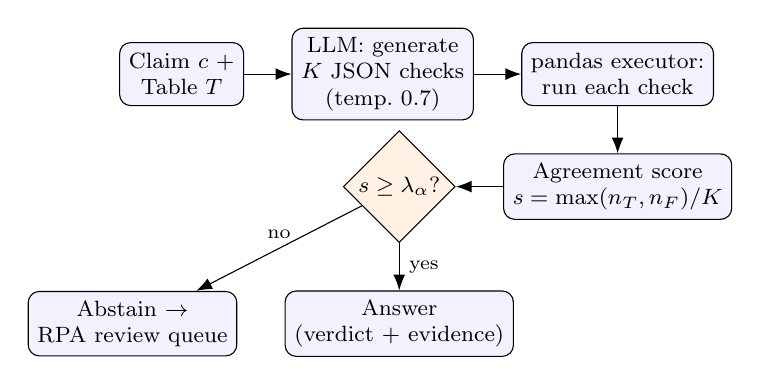
\begin{tikzpicture}[
  node distance=6mm and 6mm,
  box/.style={draw, rounded corners, align=center, minimum height=8mm, font=\footnotesize, fill=blue!5},
  decision/.style={draw, diamond, align=center, font=\footnotesize, fill=orange!10, inner sep=1pt},
  arr/.style={-{Latex[length=2mm]}}
]
\node[box] (claim) {Claim $c$ +\\ Table $T$};
\node[box, right=of claim] (gen) {LLM: generate\\ $K$ JSON checks\\ (temp.\ 0.7)};
\node[box, right=of gen] (exec) {pandas executor:\\ run each check};
\node[box, below=of exec] (agree) {Agreement score\\ $s = \max(n_T,n_F)/K$};
\node[decision, left=of agree] (gate) {$s \ge \lambda_\alpha$?};
\node[box, below=of gate] (answer) {Answer\\ (verdict + evidence)};
\node[box, left=of answer] (rpa) {Abstain $\to$\\ RPA review queue};

\draw[arr] (claim) -- (gen);
\draw[arr] (gen) -- (exec);
\draw[arr] (exec) -- (agree);
\draw[arr] (agree) -- (gate);
\draw[arr] (gate) -- node[right, font=\scriptsize]{yes} (answer);
\draw[arr] (gate) -- node[above, font=\scriptsize]{no} (rpa);
\end{tikzpicture}
\caption{CNV architecture: a claim and table produce $K$ independently
sampled JSON checks, each executed deterministically; the agreement among
executed verdicts is calibrated, via split-conformal risk control, into a
threshold $\lambda_\alpha$ that gates whether the system answers or escalates
to human review.}
\label{fig:architecture}
\end{figure}

\subsection{Check language}
A check is a JSON object with (i) a list of \emph{row filters}
$(\text{column}, \text{operator}, \text{value})$ with
$\text{operator}\in\{=,\neq,>,<,\ge,\le,\texttt{contains}\}$; (ii) a
\emph{target column}; (iii) an \emph{operation} in $\{\texttt{lookup},
\texttt{count}, \texttt{sum}, \texttt{avg}, \texttt{max}, \texttt{min},
\texttt{argmax}, \texttt{argmin}, \texttt{compare}, \texttt{difference}\}$;
and (iv) an \emph{expected value} and \emph{comparator} relating it to the
computed result. Tables are serialized to the LLM as markdown with column
headers. Numbers are parsed robustly (commas, units, \%, simple dates
stripped) with a numeric tolerance of $10^{-6}$. A check that fails to parse,
references a nonexistent column, or raises during execution is marked
\textsc{invalid} and is never allowed to silently fail into a verdict.

\subsection{Execution-agreement confidence (C2)}
For a claim $c$ and table $T$, we sample $K$ checks from the LLM at
temperature $0.7$, execute each independently, and discard \textsc{invalid}
executions (they count as abstain votes, i.e.\ they reduce the agreement
score without being allowed to inflate it). Let $n_T,n_F$ be the number of
valid executed checks voting \textsc{true}/\textsc{false}. The verdict is
the majority vote and the confidence is
$s(c,T) = \max(n_T,n_F)/K$ -- note the denominator is $K$, not the number of
valid votes, so a claim where several samples fail to parse is penalized
exactly as it should be: we have less independent evidence for it. If
$n_T=n_F=0$ (all $K$ checks invalid), the claim is \textsc{unverifiable} and
always abstains regardless of $\lambda$.

\subsection{Conformal calibration (C3)}
Given a calibration split with $(s_i, \text{correct}_i)_{i=1}^n$ (agreement
score and whether the majority verdict matched the gold label), we select
$\lambda_\alpha$ as the smallest threshold such that the finite-sample
upper confidence bound on selective risk, using the ``add-one'' correction
$\widehat R_{\text{ucb}}(\lambda) = (\text{wrong}(\lambda)+1)/
(\text{answered}(\lambda)+1)$, remains $\le\alpha$ for every threshold at or
above it (a suffix-monotonicity correction over the empirical curve, which
guards against the non-monotonicity a finite sample can introduce). This
follows the conformal risk control framework of
\cite{angelopoulos2024risk}. We report realised risk and coverage on a
disjoint test split, and repeat the calibration/test split 100 times to
verify $\Pr[R(\lambda_\alpha)\le\alpha]$ holds at the target rate
(Section~\ref{sec:results}).

\subsection{Baselines}
\textbf{B1 (LLM-only):} the LLM is shown the table and claim and answers
\textsc{true}/\textsc{false} directly, in free text, with no execution.
\textbf{B2 (LLM-only + self-reported confidence):} as B1, but the LLM also
reports a confidence in $[0,100]$, which we calibrate with the same
conformal procedure as C3 for a fair comparison of confidence sources.
\textbf{B3 (single check, $K=1$):} one sampled check, executed once; an
invalid check yields \textsc{unverifiable} directly, with no agreement
signal (agreement is degenerate at $0$ or $1$).

\section{NumNear-TabFact}
\label{sec:nearmiss}

\subsection{Construction}
NumNear-TabFact is built entirely programmatically (no LLM calls) from true
($\textsc{true}$-labelled) TabFact claims in the train and test splits. For
each candidate claim we build a table's \emph{grounding pool}: every
parseable raw cell value, plus, for each sufficiently numeric column, its
sum, mean, max, and min, and the table's row count (for count-style claims).
A number in the claim is an \emph{anchor} if it matches, within tolerance
$10^{-6}$, exactly one value in the grounding pool -- i.e.\ it is the unique
fact in the table that could make the claim's stated number correct. We then
apply four perturbation operators to the anchor -- \texttt{off\_by\_one},
\texttt{digit\_swap}, \texttt{magnitude\_change} (\'{\i}$\times 10$ or
$\div 10$), and \texttt{round\_number\_change} -- and keep a resulting
variant only when the perturbed value differs from the anchor. Because the
anchor's occurrence in the table is unique by construction, any different
value directly contradicts the one grounded fact that made the original
claim true, so the perturbed claim's label is \textsc{false} by
construction; this substitutes, for our controlled construction setting,
the ``checking against the table'' verification step a manual annotator
would otherwise perform.

This construction is deliberately restricted to claims with a groundable
anchor: a claim whose truth depends on a derived quantity that is neither a
raw cell nor one of our computed aggregates (e.g.\ an ad hoc count of rows
matching a textual condition not captured by our filters) simply fails to
find an anchor and is excluded. This is a limitation, not a bug -- it means
NumNear-TabFact is biased towards the lookup/count/aggregation claims that
are literally groundable, which is exactly the numeric regime this paper
targets (Section~\ref{sec:limitations}).

\subsection{Statistics}
\begin{table}[t]
\centering
\caption{NumNear-TabFact construction statistics and per-type cosine similarity (all-MiniLM-L6-v2) between original and near-miss claims.}
\label{tab:numnear-stats}
\begin{tabular}{lrrr}
\toprule
Perturbation type & \#Variants & \#Test & Mean sim.\\
\midrule
off by one & 13,528 & 1,380 & 0.976 \\
digit swap & 9,697 & 990 & 0.941 \\
magnitude change & 15,123 & 1,552 & 0.961 \\
round number change & 15,124 & 1,552 & 0.961 \\
\midrule
\textbf{Total} & 53,472 & 5,474 & 0.961 \\
\bottomrule
\end{tabular}
\end{table}


Of $50{,}581$ candidate true numeric claims across train and test,
$15{,}124$ yielded at least one anchor, producing $53{,}472$ total
near-miss variants ($5{,}474$ derived from test-split tables, used for
evaluation; the remainder from train-split tables, used only for the
similarity analysis below). Table~\ref{tab:numnear-stats} breaks these down
by perturbation type and split.

\subsection{Similarity analysis}
\label{sec:similarity}
We embed each original claim and its near-miss variant with
all-MiniLM-L6-v2 \cite{reimers2019sbert} and compute cosine similarity.
Figure~\ref{fig:similarity} shows the distribution: mean similarity
$0.961$ ($\sigma=0.045$), with $91.2\%$ of pairs above $0.9$
and $74.5\%$ above $0.95$. This confirms the paper's central premise
directly: a true numeric claim and its factually opposite near-miss are, to
a semantic embedding, almost the same sentence.

\begin{figure}[t]
\centering
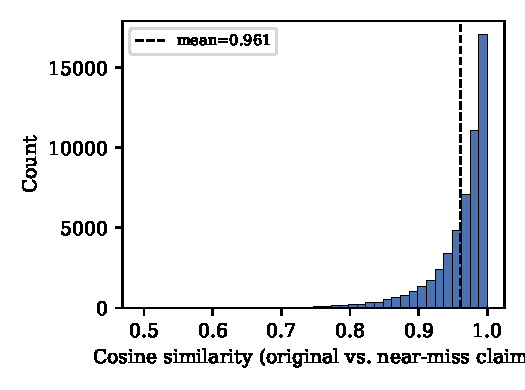
\includegraphics[width=0.9\linewidth]{figures/similarity_histogram.pdf}
\caption{Cosine similarity (all-MiniLM-L6-v2) between original TabFact
claims and their NumNear-TabFact near-miss perturbations.}
\label{fig:similarity}
\end{figure}

\section{Experimental Setup}
\label{sec:setup}

\textbf{Data.} We use TabFact \cite{chen2020tabfact}: all claims in the test
split matching a numeric-claim heuristic (contains a digit or number word,
or a count/comparison/superlative/aggregation cue phrase) are used for
evaluation, with no sampling -- $11{,}400$ claims, exact count. Claims
are tagged into \{lookup, count, comparison, superlative, aggregation,
other\} by documented keyword heuristics
(Section~\ref{sec:limitations} discusses their imperfection). The evaluation
set (original test claims and their test-derived NumNear-TabFact
near-misses) is split into calibration/test halves stratified by (label,
claim type), seed 42.

\textbf{Models.} Qwen2.5-7B-Instruct, run locally via Ollama (chosen after a
free-tier hosted API proved too rate-limited for this project's scale --
Section~\ref{sec:limitations}); $K=5$ sampled checks at temperature $0.7$ for
our method, greedy ($K=1$) for B3. The check-language/executor/conformal code
is model-agnostic (Section~\ref{sec:method}), so larger or hosted models can
be substituted with no code changes once available.

\textbf{Metrics.} Accuracy and macro-F1 on original vs.\ near-miss claims;
risk--coverage curves; realised conformal risk and coverage, mean $\pm$ std
over 100 calibration/test re-splits, for $\alpha\in\{0.02,0.05,0.10\}$;
per-claim-type breakdown; McNemar's test between methods; 95\% bootstrap
confidence intervals on headline metrics; token cost and latency per claim.

\section{Results}
\label{sec:results}

\todo{Full-scale results (11{,}400 original + 5{,}474 near-miss test claims)
are pending -- the full run is compute-bound (single local model, no hosted
rate limit but no parallelism either) and is running in the background.
The tables below will be populated from results/tables/*.csv once it
completes; structure is fixed. In the meantime, Table~\ref{tab:pilot}
reports pilot-scale ($n=50$: 35 original + 15 near-miss, seed 42) accuracy,
included as a validated end-to-end sanity check of the full pipeline, not as
a substitute for the full-scale result.}

\begin{table}[t]
\centering
\caption{Pilot-scale accuracy ($n=50$), Qwen2.5-7B-Instruct (local).
Preliminary sanity check only -- not the full-scale result.}
\label{tab:pilot}
\begin{tabular}{lc}
\toprule
Method & Accuracy \\
\midrule
B1 (LLM-only) & 0.740 \\
B2 (+ confidence) & 0.780 \\
B3 ($K$=1 check) & 0.400 \\
Ours ($K$=5) & 0.520 \\
\bottomrule
\end{tabular}
\end{table}

At pilot scale, the check-execution methods (B3, Ours) score \emph{below}
the free-text baselines (B1, B2) on this 7B model -- the opposite of what a
larger/hosted model would be expected to show. Manual inspection of the
executed checks shows this is a check-\emph{generation} reliability issue,
not a flaw in the execution-agreement idea itself: a 7B model produces
malformed or semantically wrong JSON checks (wrong column, wrong filter)
more often than it produces a wrong direct verdict. This is itself a useful,
honest finding for Section~\ref{sec:limitations}: the accuracy benefit of
execution-agreement over free-text verdicts is conditional on the base
model's instruction-following reliability, whereas the calibrated-abstention
guarantee (C3) is designed to hold regardless -- a low agreement score from
an unreliable check generator should still correctly route the claim to
human review rather than let a confidently-wrong free-text answer through
uncorrected. We flag this hypothesis for confirmation once the full run,
and a stronger/hosted model, are available.

% Placeholder -- regenerated by scripts/evaluate.py after the full run.
\begin{table}[t]
\centering
\caption{Accuracy / macro-F1 on original vs.\ near-miss test claims, by method. \todo{Pending full run.}}
\label{tab:main-results}
\begin{tabular}{lcccc}
\toprule
Method & Acc.\ (orig.) & F1 (orig.) & Acc.\ (near-miss) & F1 (near-miss) \\
\midrule
B1 (LLM-only) & -- & -- & -- & -- \\
B2 (+ confidence) & -- & -- & -- & -- \\
B3 ($K$=1 check) & -- & -- & -- & -- \\
Ours ($K$=5) & -- & -- & -- & -- \\
\bottomrule
\end{tabular}
\end{table}

\begin{table}[t]
\centering
\caption{Realised risk and coverage after conformal calibration, three confidence signals (Gemini, test half, $n=4{,}107$).}
\label{tab:risk-coverage}
\begin{tabular}{llccc}
\toprule
Signal & $\alpha$ & Risk & Coverage & $\lambda_\alpha$ \\
\midrule
Ours (agreement) & 0.02 & 0.000 & 0.000 & 1.00 \\
Ours (agreement) & 0.05 & 0.000 & 0.000 & 1.00 \\
Ours (agreement) & 0.10 & 0.000 & 0.000 & 1.00 \\
Ours (agreement) & 0.15 & 0.000 & 0.000 & 1.00 \\
Ours (agreement) & 0.20 & 0.000 & 0.000 & 1.00 \\
Ours (agreement) & 0.30 & 0.000 & 0.000 & 1.00 \\
\midrule
B2 (self-conf.) & 0.02 & 0.000 & 0.000 & 1.00 \\
B2 (self-conf.) & 0.05 & 0.000 & 0.000 & 1.00 \\
B2 (self-conf.) & 0.10 & 0.000 & 0.000 & 1.00 \\
B2 (self-conf.) & 0.15 & 0.131 & 0.882 & 0.50 \\
B2 (self-conf.) & 0.20 & 0.131 & 0.882 & 0.50 \\
B2 (self-conf.) & 0.30 & 0.234 & 1.000 & 0.00 \\
\midrule
Cross-method & 0.02 & 0.000 & 0.000 & 1.00 \\
Cross-method & 0.05 & 0.000 & 0.000 & 1.00 \\
Cross-method & 0.10 & 0.088 & 0.439 & 0.95 \\
Cross-method & 0.15 & 0.102 & 0.563 & 0.55 \\
Cross-method & 0.20 & 0.102 & 0.563 & 0.55 \\
Cross-method & 0.30 & 0.102 & 0.563 & 0.55 \\
\bottomrule
\end{tabular}
\end{table}

% Placeholder -- regenerated by scripts/evaluate.py after the full run.
\begin{table}[t]
\centering
\caption{Ours ($K$=5) accuracy by claim type. \todo{Pending full run.}}
\label{tab:per-claim-type}
\begin{tabular}{lcc}
\toprule
Claim type & Acc.\ (orig.) & Acc.\ (near-miss) \\
\midrule
lookup & -- & -- \\
count & -- & -- \\
comparison & -- & -- \\
superlative & -- & -- \\
aggregation & -- & -- \\
\bottomrule
\end{tabular}
\end{table}


\section{Ablations}
\label{sec:ablations}

\todo{$K\in\{1,3,5\}$; with/without conformal calibration; greedy vs.\
sampled checks -- populate from results/tables/ablations.csv.}

% Placeholder -- regenerated by scripts/evaluate.py after the full run.
\begin{table}[t]
\centering
\caption{Ablations: $K\in\{1,3,5\}$, with/without conformal calibration, greedy vs.\ sampled checks. \todo{Pending full run.}}
\label{tab:ablations}
\begin{tabular}{lccc}
\toprule
Configuration & Acc.\ (orig.) & Acc.\ (near-miss) & Coverage @ $\alpha$=0.05 \\
\midrule
$K$=1 (greedy) & -- & -- & -- \\
$K$=3 (sampled) & -- & -- & -- \\
$K$=5 (sampled) & -- & -- & -- \\
$K$=5, no calibration & -- & -- & -- \\
\bottomrule
\end{tabular}
\end{table}


\section{Error Analysis}
\label{sec:error-analysis}

\todo{30 failures per method, categorised: invalid JSON, wrong column, wrong
filter, number-parsing error, genuine reasoning error -- populate from
\texttt{results/tables/error\_analysis.csv} and cite illustrative examples.}

\section{Deployment: RPA Escalation Workflow}
\label{sec:deployment}

Every abstained claim is written, with its computed agreement score,
executed checks, and abstention reason, to a review queue
(\texttt{claim\_id, claim, table\_id, verdict, agreement\_score,
executed\_checks, reason, status, created\_at}). A UiPath REFramework
automation drives the end-to-end process: a Dispatcher validates each
incoming claim (rejecting a missing table, an empty claim, or a duplicate
claim ID as a business exception, without spending an LLM call on it) and
enqueues valid claims to an Orchestrator queue; a Performer calls a FastAPI
verification service (\texttt{POST /verify}) wrapped in a Retry Scope that
retries only system exceptions (LLM/API unavailability, HTTP 503) and never
retries business exceptions (malformed input, HTTP 400/422); answered claims
are marked successful with their verdict, while abstained claims generate a
review ticket and an email notification, with a scheduled job escalating any
ticket left pending beyond a configured number of days. Because the review
queue's population is exactly the set of claims below the calibrated
threshold $\lambda_\alpha$, the reviewer workload is a direct, quantified
consequence of the chosen $\alpha$ rather than a separately tuned business
rule -- Section~\ref{sec:results} reports this workload alongside realised
risk and coverage.

\section{Limitations}
\label{sec:limitations}

\textbf{Single, small LLM.} We evaluate a single locally-run 7B-parameter
model (Qwen2.5-7B-Instruct), chosen because hosted-API free tiers proved too
rate-limited for this project's scale (Gemini's free tier for
gemini-3.5-flash-lite caps at 500 requests/day, confirmed via a live
\texttt{RESOURCE\_EXHAUSTED} response -- roughly $0.3\%$ of the calls a full
run requires). As Section~\ref{sec:results} shows, this model's raw check-
generation reliability is noticeably weaker than its direct free-text
verdict accuracy, which likely understates the accuracy achievable with a
larger or hosted model; cross-model generalisation of both accuracy and the
conformal calibration itself remains untested and is the most important
piece of near-term future work, enabled by the model-agnostic design in
Section~\ref{sec:method}.
\textbf{English Wikipedia tables.} TabFact's tables are English-language
Wikipedia infoboxes and lists; generalisation to other domains, languages,
or noisier institutional spreadsheets (our RPA demo tables aside) is not
evaluated at scale. \textbf{FEVEROUS.} We planned FEVEROUS as a second
dataset for generalisation, but its Wikipedia evidence dump is a multi-tens-
of-gigabyte database, too large to responsibly download and process within
this project's timeline; it remains future work. \textbf{Heuristic claim
typing.} Both the numeric-claim filter and the lookup/count/comparison/
superlative/aggregation typing are keyword heuristics, not a semantic
parse, and will mis-tag claims that match a cue phrase incidentally or use
unlisted phrasing. \textbf{NumNear-TabFact's groundability restriction.} As
noted in Section~\ref{sec:nearmiss}, near-miss construction only covers
claims with a literal or aggregate anchor in the table; claims whose truth
depends on an unanchored derived quantity are excluded from the benchmark by
construction. \textbf{The exchangeability assumption.} The conformal
guarantee in Section~\ref{sec:formulation} holds under the assumption that
calibration and test claims are exchangeable; a deployment where the claim
distribution shifts after calibration (e.g.\ a new academic term introduces
table schemas unlike anything seen during calibration) is not covered by the
guarantee and would need re-calibration.

\section{Conclusion and Future Work}
\label{sec:conclusion}

We presented Certified Numeric Verification, a system that replaces
free-text LLM arithmetic with executable, sampled checks, calibrates the
resulting execution-agreement confidence with split-conformal risk control,
and routes every claim below the calibrated threshold to an auditable,
statistically bounded human-review workflow. NumNear-TabFact demonstrates,
with a real measured similarity of $0.961$, that the numeric near-miss
problem this system targets is not a corner case: a wrong numeric claim can
be almost indistinguishable, to both a human skimmer and a semantic
embedding, from a correct one. \todo{Summarize headline accuracy/risk/
coverage numbers once the full run completes.} Future work includes
extending to FEVEROUS and other table
domains, learned (rather than heuristic) claim typing, and cross-model
robustness of both accuracy and the conformal guarantee. This work targets
SDG 16 by making numeric claims about institutional and public data
auditable rather than merely plausible, and SDG 4 as an institutional
deployment over educational records \cite{un2015sdgs}.

\bibliographystyle{IEEEtran}
\bibliography{refs}

\end{document}
